\documentclass[11pt,compress,t,notes=noshow, xcolor=table]{beamer}
\usepackage[]{graphicx}\usepackage[]{color}
% maxwidth is the original width if it is less than linewidth
% otherwise use linewidth (to make sure the graphics do not exceed the margin)
\makeatletter
\def\maxwidth{ %
  \ifdim\Gin@nat@width>\linewidth
    \linewidth
  \else
    \Gin@nat@width
  \fi
}
\makeatother

\newcommand{\citebutton}[2]{%
\beamergotobutton{\href{#2}{#1}}%
}

\newcommand{\blu}[1]{\textcolor{blue}{#1}}
\newcommand{\org}[1]{\textcolor{orange}{#1}}
\newcommand{\ques}{\textbf{\textcolor{red}{Question:  }}}
\newcommand{\questionssofar}{\begin{frame}\frametitle{Any questions?}\end{frame}}

\newcommand\warning{%
 \makebox[1.4em][c]{%
 \makebox[0pt][c]{\raisebox{.1em}{\scriptsize!}}%
 \makebox[0pt][c]{\color{red}\normalsize$\bigtriangleup$}}}%

\definecolor{fgcolor}{rgb}{0.345, 0.345, 0.345}
\newcommand{\hlnum}[1]{\textcolor[rgb]{0.686,0.059,0.569}{#1}}%
\newcommand{\hlstr}[1]{\textcolor[rgb]{0.192,0.494,0.8}{#1}}%
\newcommand{\hlcom}[1]{\textcolor[rgb]{0.678,0.584,0.686}{\textit{#1}}}%
\newcommand{\hlopt}[1]{\textcolor[rgb]{0,0,0}{#1}}%
\newcommand{\hlstd}[1]{\textcolor[rgb]{0.345,0.345,0.345}{#1}}%
\newcommand{\hlkwa}[1]{\textcolor[rgb]{0.161,0.373,0.58}{\textbf{#1}}}%
\newcommand{\hlkwb}[1]{\textcolor[rgb]{0.69,0.353,0.396}{#1}}%
\newcommand{\hlkwc}[1]{\textcolor[rgb]{0.333,0.667,0.333}{#1}}%
\newcommand{\hlkwd}[1]{\textcolor[rgb]{0.737,0.353,0.396}{\textbf{#1}}}%
\let\hlipl\hlkwb

\usepackage{framed}
\makeatletter
\newenvironment{kframe}{%
 \def\at@end@of@kframe{}%
 \ifinner\ifhmode%
  \def\at@end@of@kframe{\end{minipage}}%
  \begin{minipage}{\columnwidth}%
 \fi\fi%
 \def\FrameCommand##1{\hskip\@totalleftmargin \hskip-\fboxsep
 \colorbox{shadecolor}{##1}\hskip-\fboxsep
     % There is no \\@totalrightmargin, so:
     \hskip-\linewidth \hskip-\@totalleftmargin \hskip\columnwidth}%
 \MakeFramed {\advance\hsize-\width
   \@totalleftmargin\z@ \linewidth\hsize
   \@setminipage}}%
 {\par\unskip\endMakeFramed%
 \at@end@of@kframe}
\makeatother

\definecolor{shadecolor}{rgb}{.97, .97, .97}
\definecolor{messagecolor}{rgb}{0, 0, 0}
\definecolor{warningcolor}{rgb}{1, 0, 1}
\definecolor{errorcolor}{rgb}{1, 0, 0}
\newenvironment{knitrout}{}{} % an empty environment to be redefined in TeX

\usepackage{alltt}
\newcommand{\SweaveOpts}[1]{}  % do not interfere with LaTeX
\newcommand{\SweaveInput}[1]{} % because they are not real TeX commands
\newcommand{\Sexpr}[1]{}       % will only be parsed by R
\newcommand{\xmark}{\ding{55}}%


\usepackage[english]{babel}
\usepackage[utf8]{inputenc}

\usepackage{dsfont}
\usepackage{verbatim}
\usepackage{amsmath}
\usepackage{amsfonts}
\usepackage{amssymb}
\usepackage{bm}
\usepackage{csquotes}
\usepackage{multirow}
\usepackage{longtable}
\usepackage{booktabs}
\usepackage{enumerate}
\usepackage[absolute,overlay]{textpos}
\usepackage{psfrag}
\usepackage{algorithm}
\usepackage{algpseudocode}
\usepackage{eqnarray}
\usepackage{arydshln}
\usepackage{tabularx}
\usepackage{placeins}
\usepackage{tikz}
\usepackage{setspace}
\usepackage{colortbl}
\usepackage{mathtools}
\usepackage{wrapfig}
\usepackage{bm}
\usepackage{amsmath}
\usepackage{pifont}

\usetikzlibrary{shapes.multipart,shapes,arrows,automata,positioning,calc,chains,trees, shadows}
\tikzset{
  %Define standard arrow tip
  >=stealth',
  %Define style for boxes
  punkt/.style={
    rectangle,
    rounded corners,
    draw=black, very thick,
    text width=6.5em,
    minimum height=2em,
    text centered},
  % Define arrow style
  pil/.style={
    ->,
    thick,
    shorten <=2pt,
    shorten >=2pt,}
}

\tikzstyle{vec}=[draw, rectangle, fill = white, minimum width=5mm, minimum height=1cm, inner sep = 2pt]

\usepackage{subfig}

% Defines macros and environments
\usepackage{../../style/lmu-lecture}


\let\code=\texttt
\let\proglang=\textsf

\setkeys{Gin}{width=0.9\textwidth}

\setbeamertemplate{frametitle}{\expandafter\uppercase\expandafter\insertframetitle}

\usepackage{bbm}
% basic latex stuff
\newcommand{\pkg}[1]{{\fontseries{b}\selectfont #1}} %fontstyle for R packages
\newcommand{\lz}{\vspace{0.5cm}} %vertical space
\newcommand{\dlz}{\vspace{1cm}} %double vertical space
\newcommand{\oneliner}[1] % Oneliner for important statements
{\begin{block}{}\begin{center}\begin{Large}#1\end{Large}\end{center}\end{block}}


%new environments
\newenvironment{vbframe}  %frame with breaks and verbatim
{
 \begin{frame}[containsverbatim,allowframebreaks]
}
{
\end{frame}
}

\newenvironment{vframe}  %frame with verbatim without breaks (to avoid numbering one slided frames)
{
 \begin{frame}[containsverbatim]
}
{
\end{frame}
}

\newenvironment{blocki}[1]   % itemize block
{
 \begin{block}{#1}\begin{itemize}
}
{
\end{itemize}\end{block}
}

\newenvironment{fragileframe}[2]{  %fragile frame with framebreaks
\begin{frame}[allowframebreaks, fragile, environment = fragileframe]
\frametitle{#1}
#2}
{\end{frame}}


\newcommand{\myframe}[2]{  %short for frame with framebreaks
\begin{frame}[allowframebreaks]
\frametitle{#1}
#2
\end{frame}}

\newcommand{\remark}[1]{
  \textbf{Remark:} #1
}


\newenvironment{deleteframe}
{
\begingroup
\usebackgroundtemplate{
\includegraphics[width=\paperwidth,height=\paperheight]{../style/color/red.png}}
 \begin{frame}
}
{
\end{frame}
\endgroup
}
\newenvironment{simplifyframe}
{
\begingroup
\usebackgroundtemplate{
\includegraphics[width=\paperwidth,height=\paperheight]{../style/color/yellow.png}}
 \begin{frame}
}
{
\end{frame}
\endgroup
}\newenvironment{draftframe}
{
\begingroup
\usebackgroundtemplate{
\includegraphics[width=\paperwidth,height=\paperheight]{../style/color/green.jpg}}
 \begin{frame}
}
{
\end{frame}
\endgroup
}
% https://tex.stackexchange.com/a/261480: textcolor that works in mathmode
\makeatletter
\renewcommand*{\@textcolor}[3]{%
  \protect\leavevmode
  \begingroup
    \color#1{#2}#3%
  \endgroup
}
\makeatother





\input{../../latex-math/basic-math.tex}
\input{../../latex-math/basic-ml.tex}

\newcommand{\titlefigure}{figure/arlm-mlm.png}
\newcommand{\learninggoals}{
\item Understand the concept of self-supervision
\item Gain ability to distinguish different types of language models}

\title{BERT}
% \author{}
\institute{\href{https://slds-lmu.github.io/lecture_dl4nlp/}{slds-lmu.github.io/lecture\_dl4nlp}}
\date{}

\begin{document}
\lecturechapter{ARLMs vs. MLM}
\lecture{Deep Learning for NLP} % stays constant

% ------------------------------------------------------------------------------

\begin{vbframe}{again: what is a language model?}

\vfill

\begin{itemize}
	\item Statistical model that predicts text that fits well for a given context (typically also text)
	\item Auto-regressive LMs (ARLMs)
	\begin{itemize}
		\item Predict one word that is highly likely given a prompt (previous words)
		\item For predicting an entire text, repeat the process (i.e., extend the prompt with previously predicted words)
		\item To predict a text from scratch, use an extra symbol \texttt{<START>} as the initial prompt
	\end{itemize}
\end{itemize}

\vfill

\end{vbframe}

% ------------------------------------------------------------------------------

\begin{frame}{arlm: toy example}
	\vfill
	\begin{figure}
		\centering
		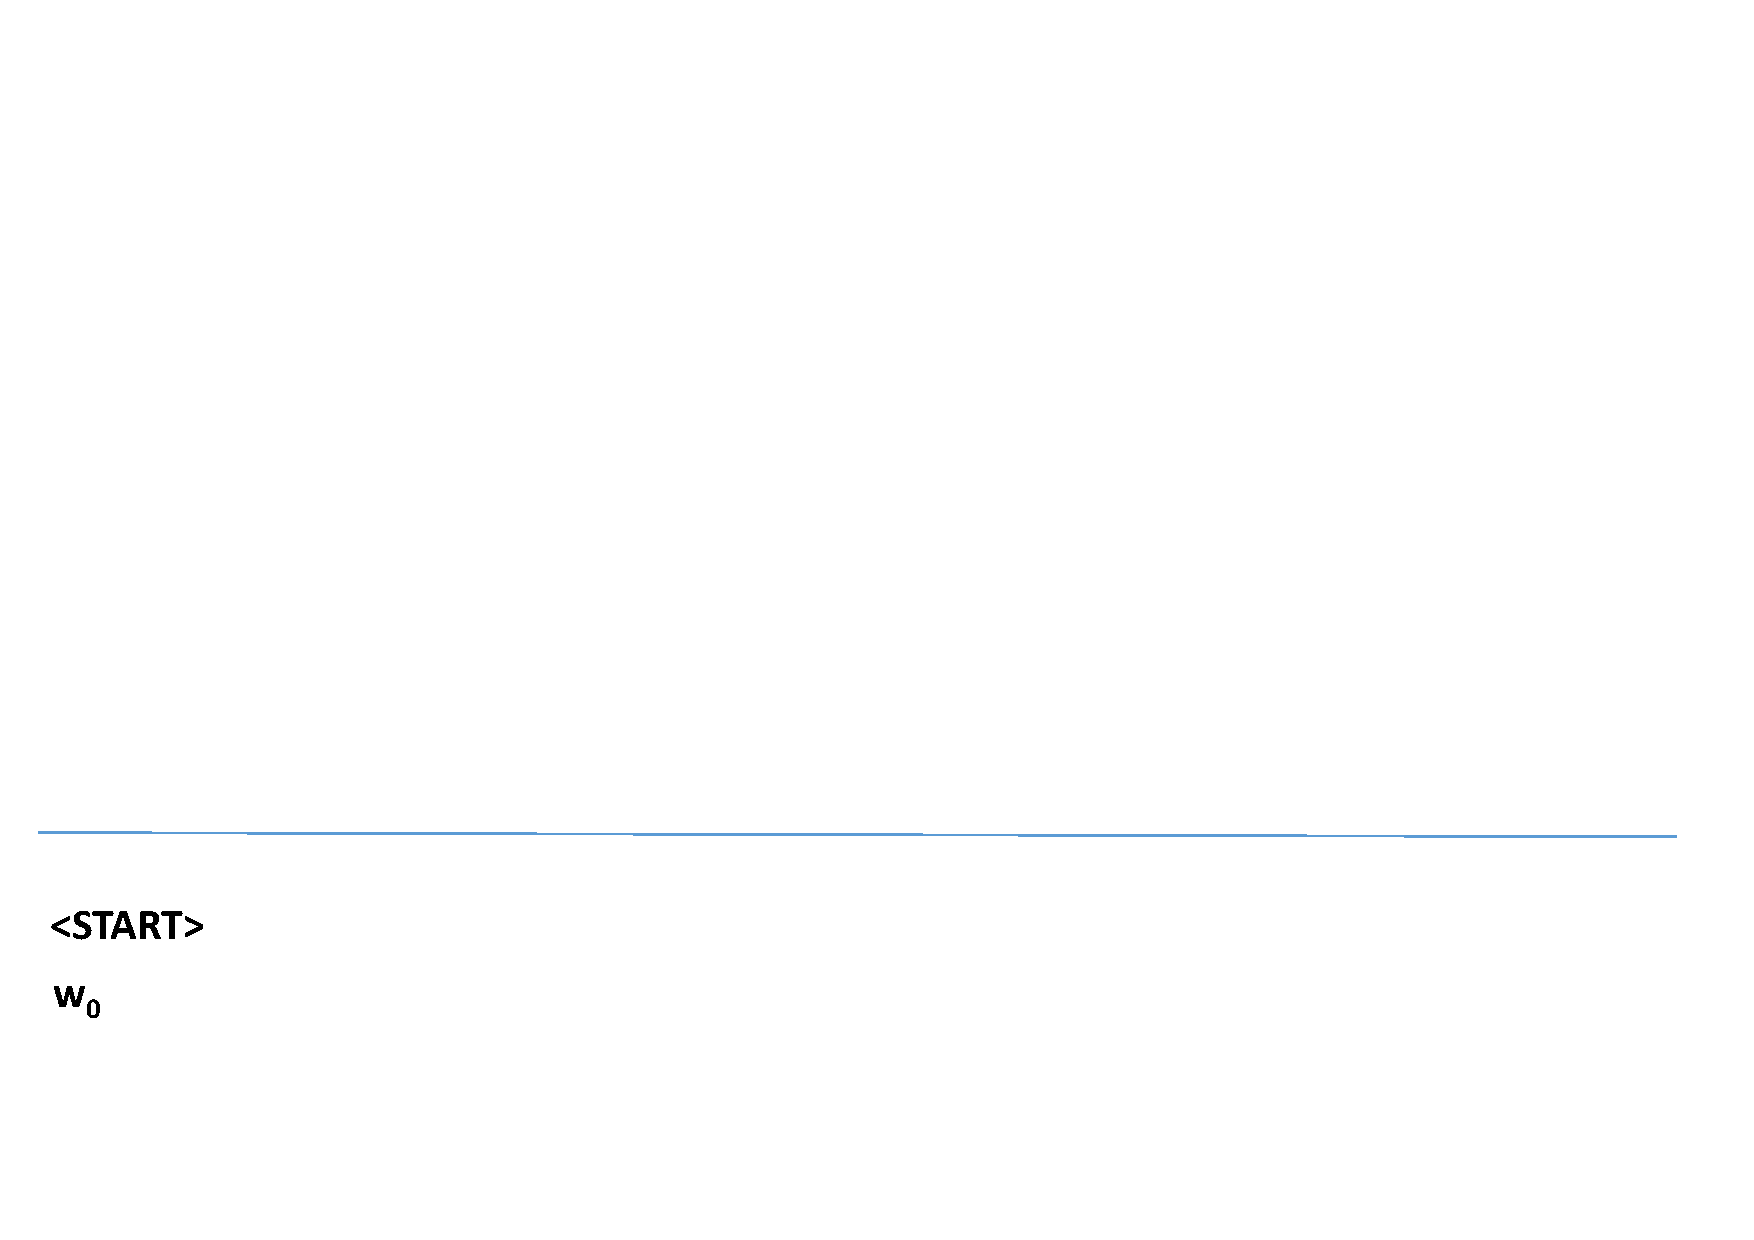
\includegraphics[width=12cm,page=1]{figure/arlm.pdf}
	\end{figure}
	\vfill
\end{frame}
\begin{frame}[noframenumbering]{arlm: toy example}
	\vfill
	\begin{figure}
		\centering
		\includegraphics[width=12cm,page=2]{figure/arlm.pdf}
	\end{figure}
	\vfill
\end{frame}
\begin{frame}[noframenumbering]{arlm: toy example}
	\vfill
	\begin{figure}
		\centering
		\includegraphics[width=12cm,page=3]{figure/arlm.pdf}
	\end{figure}
	\vfill
\end{frame}
\begin{frame}[noframenumbering]{arlm: toy example}
	\vfill
	\begin{figure}
		\centering
		\includegraphics[width=12cm,page=4]{figure/arlm.pdf}
	\end{figure}
	\vfill
\end{frame}
\begin{frame}[noframenumbering]{arlm: toy example}
	\vfill
	\begin{figure}
		\centering
		\includegraphics[width=12cm,page=5]{figure/arlm.pdf}
	\end{figure}
	\vfill
\end{frame}
\begin{frame}[noframenumbering]{arlm: toy example}
	\vfill
	\begin{figure}
		\centering
		\includegraphics[width=12cm,page=6]{figure/arlm.pdf}
	\end{figure}
	\vfill
\end{frame}
\begin{frame}[noframenumbering]{arlm: toy example}
	\vfill
	\begin{figure}
		\centering
		\includegraphics[width=12cm,page=7]{figure/arlm.pdf}
	\end{figure}
	\vfill
\end{frame}
\begin{frame}[noframenumbering]{arlm: toy example}
	\vfill
	\begin{figure}
		\centering
		\includegraphics[width=12cm,page=8]{figure/arlm.pdf}
	\end{figure}
	\vfill
\end{frame}
\begin{frame}[noframenumbering]{arlm: toy example}
	\vfill
	\begin{figure}
		\centering
		\includegraphics[width=12cm,page=9]{figure/arlm.pdf}
	\end{figure}
	\vfill
\end{frame}
\begin{frame}[noframenumbering]{arlm: toy example}
	\vfill
	\begin{figure}
		\centering
		\includegraphics[width=12cm,page=10]{figure/arlm.pdf}
	\end{figure}
	\vfill
\end{frame}
\begin{frame}[noframenumbering]{arlm: toy example}
	\vfill
	\begin{figure}
		\centering
		\includegraphics[width=12cm,page=11]{figure/arlm.pdf}
	\end{figure}
	\vfill
\end{frame}
\begin{frame}[noframenumbering]{arlm: toy example}
	\vfill
	\begin{figure}
		\centering
		\includegraphics[width=12cm,page=12]{figure/arlm.pdf}
	\end{figure}
	\vfill
\end{frame}
\begin{frame}[noframenumbering]{arlm: toy example}
	\vfill
	
	\begin{figure}
		\centering
		\includegraphics[width=12cm,page=13]{figure/arlm.pdf}
	\end{figure}
	
	\vfill
\end{frame}

% ------------------------------------------------------------------------------

\begin{vbframe}{arlm: probabilistic interpretation}

\vfill

\begin{itemize}
	\item Gives an estimate for the probability of a sentence using conditional probabilities
	\item In general: $$ P(A \cap B) = P(B) \cdot P(A | B)$$
	\item For $P(sentence)$:
	$$ P(w_1, w_2, \dots, w_n | w_0)$$ $$ = P(w_1 | w_0) \cdot P(w_2 | w_0, w_1) \cdot \hdots \cdot P(w_n | w_0, \dots, w_{n-1})$$
\end{itemize}

\vfill

\end{vbframe}


% ------------------------------------------------------------------------------

\begin{vbframe}{Examples of ARLMs (1)}

\vfill

\textbf{Neural Machine Translation:}

	\begin{figure}
		\centering
		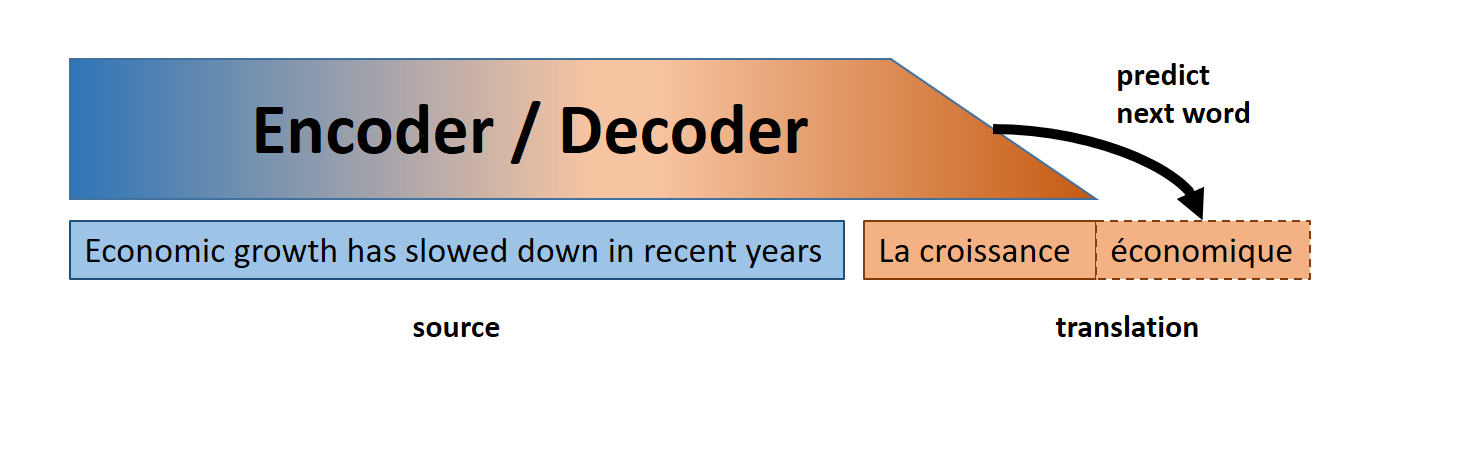
\includegraphics[width=12cm]{figure/arlm1.png}
	\end{figure}
	
\vfill

\end{vbframe}

% ------------------------------------------------------------------------------

\begin{vbframe}{Examples of ARLMs (1)}

\vfill

\textbf{Image Captioning:}

	\begin{figure}
		\centering
		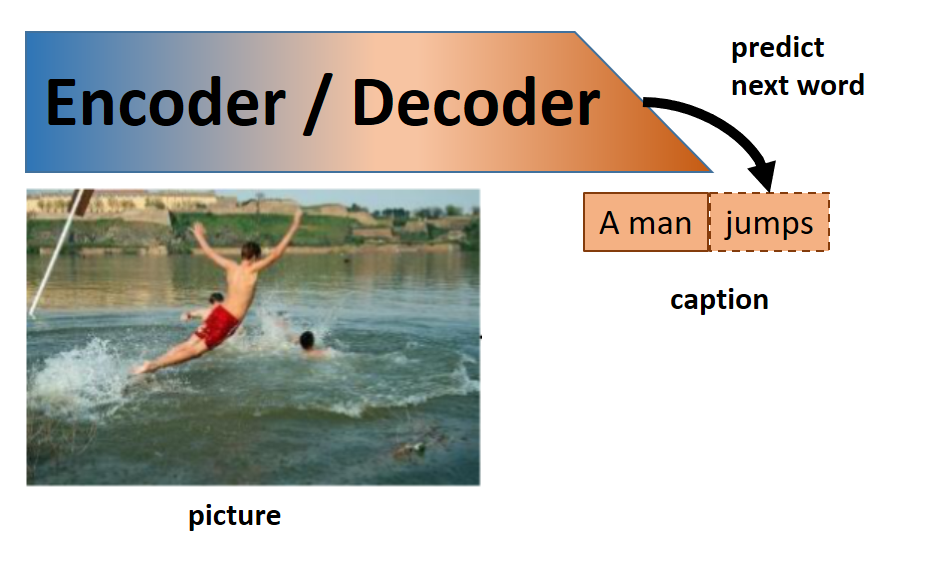
\includegraphics[width=8cm]{figure/arlm2.png}
	\end{figure}
\vfill

\end{vbframe}

% ------------------------------------------------------------------------------

\begin{vbframe}{Masked language models (MLM)}

\vfill

\begin{itemize}
	\item We have seen auto-regressive LMs
			\begin{itemize}
				\item context: previous words
				\item predict: next word
			\end{itemize}
	\item Another type: \textit{Masked} LMs (MLMs)
			\begin{itemize}
				\item context: surrounding words
				\item predict: masked word
			\end{itemize}
\end{itemize}

\vfill

\end{vbframe}

% ------------------------------------------------------------------------------

\begin{vbframe}{mlm: toy example}

\vfill

	\begin{figure}
		\centering
		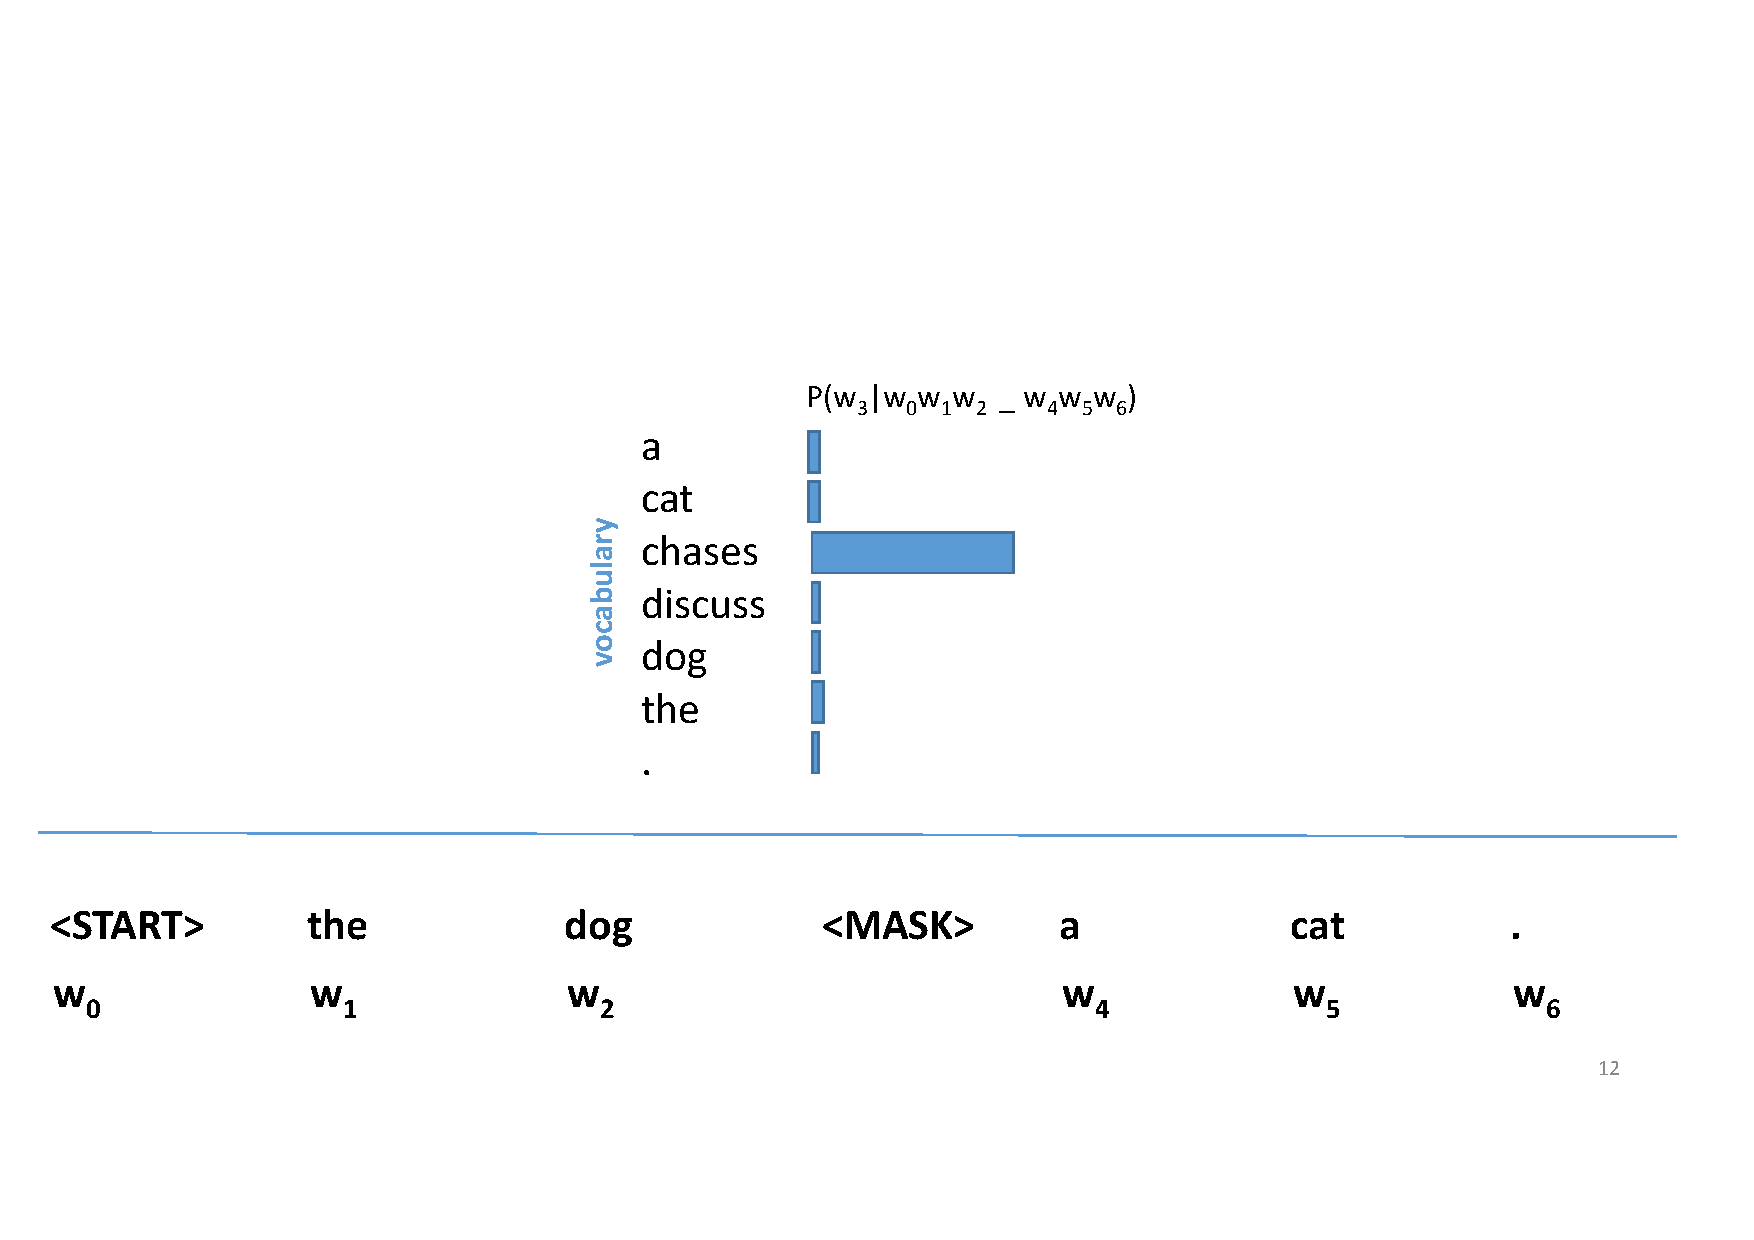
\includegraphics[width=10cm]{figure/mlm.pdf}
	\end{figure}
	
\vfill

\end{vbframe}

% ------------------------------------------------------------------------------

\begin{vbframe}{mlm: probabilistic interpretation}

\vfill

\begin{itemize}
	\item Estimates $P(w_i | w_0, w_1, w_{i-1}, \dots, w_{i+1}, w_n)$
	\item No ``clean`` estimate for $P(sentence)$, as
	$$ P(w_1, w_2, \dots, w_n | w_0)$$ $$\neq P(w_1 | w_0, w_2, \dots, w_n) \cdot P(w_2 | w_0, w_1, w_3, \dots, w_n)$$
	\item ARLMs are better than MLMs for generating texts 
	\item Advantage of MLMs: Learning contextualized representations
\end{itemize}

\vfill

\end{vbframe}

% ------------------------------------------------------------------------------

\begin{vbframe}{self-supervision}

\vfill

	\begin{figure}
		\centering
		
\includegraphics[width=10cm]{figure/selfsup.jpeg}
	\end{figure}
	
\vfill

\end{vbframe}

% ------------------------------------------------------------------------------

\begin{frame}{Definition}

	\vfill 
	
	\textit{Unsupervised Learning:}

	\begin{itemize}
		\item No labels attached to the data
		\item Learn patterns / clusters from the features only
	\end{itemize}
	
	\textit{Supervised Learning:}

	\begin{itemize}
		\item (Gold) Labels attached to the data
		\item Learn from the association between features and labels
	\end{itemize}
	
	\textbf{Self-Supervised Learning:}

	\begin{itemize}
		\item No \textit{external} labels attached to the data\\
					$\to$ Samples with suitable labels can be generated from the known structure of the data itself 
		\item \textit{Technically} supervised learning, but \textit{no labeling effort} $+$ simultan-\\eous ability to generate massive amounts of labeled data points
	\end{itemize}
	
	\vfill 
	
\end{frame}

% ------------------------------------------------------------------------------

\begin{vbframe}{Self-supervised objectives}

\vfill

\textbf{Self-supervised objectives:}
	
	\begin{itemize}
		\item Skip-gram objective (cf. word2vec)
		\item Language modeling objective
		\item \textit{Masked language modeling (MLM)} objective
		\item ... and many more possibilities for text data
	\end{itemize}
\vfill

\end{vbframe}

% ------------------------------------------------------------------------------

\endlecture
\end{document}